\newpage
\genHeader
\hypertarget{remCard end}{}
\subsubsection{Concluding removeCard}

Let's take a step back and briefly review what we have specified:  if \texttt{p.remove\-Card(c)} is invoked for a partition \texttt{p}, with a card, \texttt{c},
as its argument, the specified pattern will \emph{match} only if that card is contained in the partition. After determining matches for all variables, the
link between the partition and the card is deleted, effectively ``removing'' the card from the partition. If the card is \emph{not} contained in the partition,
the pattern won't match, and nothing will happen. In both cases, the card that's passed in is returned.

\begin{itemize}

\item[$\blacktriangleright$] If your code generation was successful, navigate to 
``Learning\-Box\-Language/\-gen/\-Learning\-Box\-Language/\-impl/\-Partition\-Impl.java" to the \texttt{\-remove\-Card} declaration (approximately line 385).
Inspect the generated implementation for your method (Fig.~\ref{fig:remCardImpl}). Notice all the null checks that are automatically created - only a very conscientious
(and probably slightly paranoid) programmer would program so defensively!

\begin{figure}[htp]
\begin{center}
  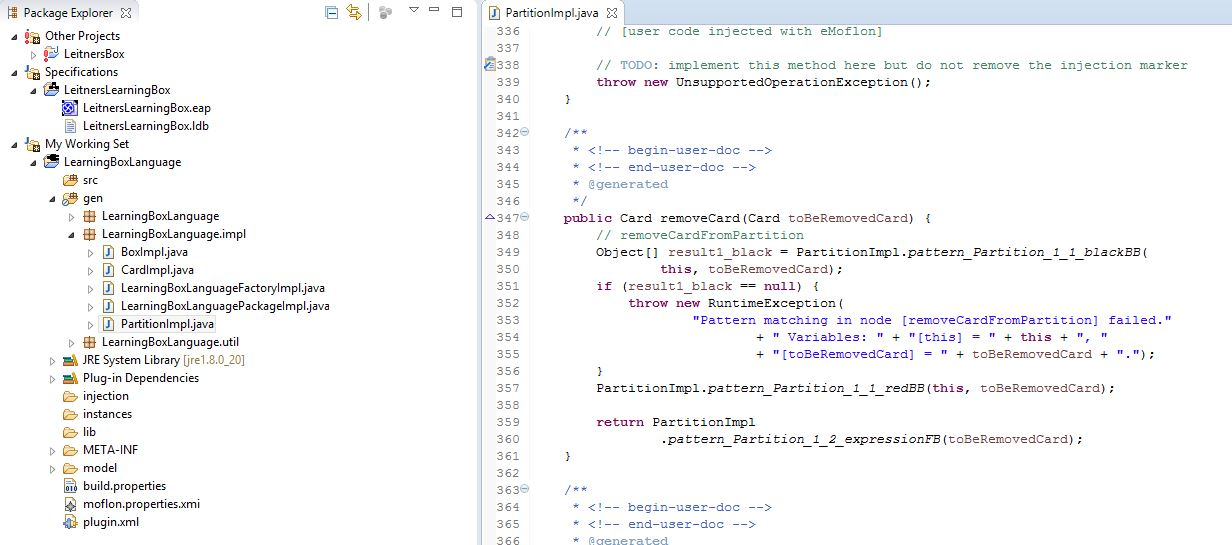
\includegraphics[width=\textwidth]{eclipse_remCardImpl}
  \caption{Generated implementation code}
  \label{fig:remCardImpl}
\end{center}
\end{figure}

\item[$\blacktriangleright$] After using injections, you were able to test your implementation with \texttt{LeitnersBoxGui},\footnote{If you haven't downloaded
or used the GUI before, review Part II, Section 7} so lets test and make sure \emph{this} version works. Load and run the GUI, then go to any partition and
select \texttt{Remove Card}. If it doesn't work, make sure your metamodel is built, and double check your specification syntax.

\end{itemize}